\documentclass[letterpaper]{article}

%%%%% Math
\usepackage{amssymb}
\usepackage{mathtools}
\usepackage{mathrsfs}
\newcommand{\defequal}{\mathrel{\overset{\makebox[0pt]{\mbox{\tiny def}}}{=}}}
\newcommand{\E}{\mathbb{E}} % Expectation
\newcommand{\1}{\mathbb{I} } % indicator with no arguments
\newcommand{\indic}[1]{\1_{#1}} % indicator function
\DeclareMathOperator*{\argmax}{\arg\max}
\DeclareMathOperator*{\argmin}{\arg\min}
%%%%% End: Math

%%%%%% ALife conf recommendation
\usepackage{natbib}
\usepackage{alifeconf}
\usepackage{url}
\usepackage{booktabs}
\usepackage{hyperref}
\usepackage{cleveref}
%%%%%% End: ALife conf recommendation

%%%%% Caption
\usepackage[bf]{caption}
\usepackage{subcaption}
\usepackage[space]{grffile}
%%%%% End: Graphics

%%%%% Hyperref
\usepackage{xcolor}
\definecolor{dark-blue}{rgb}{0.05,0.1,0.75}
\hypersetup{
  colorlinks,
  linkcolor={dark-blue},
  citecolor={dark-blue},
  urlcolor={dark-blue}
}
%%%%% End: Hyperref

%%%%%% Cut padding
\setlength{\belowcaptionskip}{-10pt}
\setlength{\abovedisplayskip}{1pt}
\setlength{\belowdisplayskip}{3pt}
%%%%% End: Cut padding

%%%%%% Todo utilities
\usepackage{todonotes}
\setuptodonotes{
  inline,
  linecolor=blue,
  backgroundcolor=blue,
  textcolor=white,
  bordercolor=blue,
}
%%%%% End: Todo utilities

%%%%% Roman number
\newcounter{num}
\newcommand{\rnum}[1]{\setcounter{num}{#1}(\roman{num})}
%%%%% End: Roman number

%%%%% MDP
\newcommand{\M}{\mathcal{M}} % MDP
\newcommand{\A}{\mathcal{A}} % Actions
\newcommand{\X}{\mathcal{S}} % States
\newcommand{\ah}{\hat{A}} % Estimation of Advantage
\newcommand{\vh}{\hat{V}} % Estimation of Value
%%%%% End: MDP

%%%%% Table
\usepackage{siunitx}
\usepackage{longtable} % tables that can span several pages
%%%%% End: Table

%%%%% Graphics
\graphicspath{{./resources}} % Specifies the directory where pictures are stored
%%%%% End: Graphics

%%%%% Pseudo codes
\usepackage[indLines=false]{algpseudocodex}
\usepackage{algorithm}
\makeatletter
\algnewcommand\algorithmiconce{\textbf{Once}}%
\algdef{SE}[ONCE]{Once}{EndOnce}[1]{\algpx@startIndent\algpx@startCodeCommand\algorithmiconce\ #1\ \algorithmicdo%
}{\algpx@endIndent\algpx@startEndBlockCommand\algorithmicend\ \algorithmiconce}%
\pretocmd{\Once}{\algpx@endCodeCommand}{}{}
\algtext*{EndOnce}%
\apptocmd{\EndOnce}{\algpx@endIndent}{}{}%
\pretocmd{\EndOnce}{\algpx@endCodeCommand[1]}{}{}%

\algnewcommand\algorithmicWith{\textbf{With}}%
\algdef{SE}[WITH]{With}{EndWith}[1]{\algpx@startIndent\algpx@startCodeCommand\algorithmicWith\ #1\ \algorithmicdo%
}{\algpx@endIndent\algpx@startEndBlockCommand\algorithmicend\ \algorithmicWith}%
\pretocmd{\With}{\algpx@endCodeCommand}{}{}
\algtext*{EndWith}%
\apptocmd{\EndWith}{\algpx@endIndent}{}{}%
\pretocmd{\EndWith}{\algpx@endCodeCommand[1]}{}{}%
\makeatother
%%%%% End: Pseudo Codes

\title{On the Dynamics of Food Reward and Fatigue in Distributed Evolution}
\author{
  Anonymous authors
  % Yuji Kanagawa$^{1}$ \and
  % Kenji Doya$^{1}$ \\
  % \mbox{}\\
  % $^1$Okinawa Institute of Science and Technology Graduate University, Japan
  % yuji.kanagawa@oist.jp
} % email of corresponding author

%%%%%%%%%%%%%%%%%%%%%%%%%%%%%%%%%%%%%%%%%%%%%%%%%%%%%%%%%%%%%%%%
%% Begin document, create title and abstract
%%%%%%%%%%%%%%%%%%%%%%%%%%%%%%%%%%%%%%%%%%%%%%%%%%%%%%%%%%%%%%%%
\begin{document}

\maketitle

\begin{abstract}
  The reward system is one of the fundamental drivers of animal behaviors and is critical for survival and reproduction. Despite its importance, the problem of how the reward system has evolved is underexplored. In this paper, we investigate in what environmental conditions biologically plausible reward functions evolve. For this purpose, we developed a population-based decentralized evolutionary simulation framework, where agents need to maintain their energy level to live longer and produce more children. Each agent inherits its reward function from its parent subject to mutation and learns to get rewards via reinforcement learning throughout its lifetime. Our results show that biologically reasonable positive rewards for food acquisition and negative rewards for motor exertion can evolve from randomly initialized ones. However, we also find that the reward for taking motor action can be unstable and vary depending on the environment. In environments with poor and poisonous foods, the evolution of rewards for less important foods tends to be unstable, while rewards for normal foods are still stable.
  These results demonstrate the usefulness of our energy-dependent life-death-reproduction model for further studies of the origin of reward systems.
\end{abstract}

\section{Introduction}\label{sec:intro}
Producing reward signals is a fundamental animal brain function to live and reproduce. Positive rewards, such as pleasure, encourage us to eat and find partners, while negative rewards, such as fatigue, help us protect ourselves. These reward signals affect our behavior through learning. Our brain produces a reward signal to a specific stimulus, such as good food, reinforcing our behavior to get more rewards. This mechanism, called reinforcement learning (RL), has been extensively studied in neuroscience and computer science. Neuroscientists have revealed that our brain has some hot or cold spots that respond to good or bad events~\citep{berridgeAffectiveNeurosciencePleasure2008}, and how those signals are used for learning~\citep{schultzNeuronalRewardDecision2015}, while computational reinforcement learning has provided theoretical models and several applications including game-playing agents and robotics~\citep{suttonReinforcementLearningIntroduction2018}.

% Problem: Reward evolution
% Why this topic has been underexplored, and how we can find some interesting points from this line of research
Due to its significant contribution to our lives, how our reward system has evolved is an interesting open question. A common explanation is based on natural selection, arguing that rewards have evolved to help animals survive in the environment and successfully reproduce offspring (e.g., by~\cite{schultzNeuronalRewardDecision2015}). While this hypothesis sounds reasonable, it is unclear what kind of environmental condition triggered the evolution of rewards. Another question is how the characteristics of our current rewards have evolved, such as food reward regulation by satiety.

% Importance of simulation
While biological studies on evolutionary biology and neuroscience are essential in addressing these questions, we argue that computational study can contribute to this area by providing a simplified model of natural evolution. A good example is the relationship between biological and computational RL, which have evolved closely. While computational RL has provided us with helpful engineering techniques, it has also provided a promising computational model for how animals learn. We aim to make a similar contribution to the problem of reward evolution.

% Why the population-based model is important
For this purpose, we propose to use a population-based distributed evolution framework to simulate the evolution of rewards. Classical studies on the evolution of learning \citep{hintonHowLearningCan1987,singhWhereRewardsCome2009} often employ a centralized evolution scheme where some tightly evaluated elites are selected as parents. While this approach is simple and computationally efficient, it somewhat sacrifices the biological reality. Instead, our simulation model employs birth and death conditions for each agent and lets evolution happen locally. Each agent inherits a reward function from its parent and learns to get more rewards during its lifetime. Through this process, we expect that naturalistic reward functions will evolve.

\section{Preliminaries and Related Works}\label{sec:related}
We follow the standard computational RL framework \citep{suttonReinforcementLearningIntroduction2018} based on the Markov decision process (MDP). MDP $\M{}$ consists of a tuple $(\X{}, \A{}, p, r, \gamma)$, where $\X{}$ is state space, $\A{}$ is action space, $p: \X\times\A\times \X \rightarrow [0, 1]$ is state transition function, $r: \X\times\A \rightarrow \mathcal{R}$ is reward function, and $\gamma \in [0, 1]$ is the discount factor. A standard objective in MDP is the discounted cumulative return $G \defequal{} \sum_{t=0}^{\infty}\gamma^t R_{t}$, where $R_t$ is the reward received at time $t$. An RL agent has policy $\pi: \X \times \A \rightarrow [0, 1]$ and seeks to find the the optimal policy $\pi^{*}$ that maximizes $\E \left[G|\pi\right]$. The state-value function $V^\pi(s) \defequal \sum_{a \in \A} \pi(a|s) \left( r(s, a) + \gamma \sum_{s' \in \X} P(s'|s, a) V^\pi(s') \right)$ is often used in RL algorithms. Observation $o \in \Omega~(\Omega \subseteq \X)$ often refers to a part of the state that an agent can observe.

Our reward model is inspired by the neuroscience of reward system \citep{schultzNeuronalRewardDecision2015, berridgePleasureSystemsBrain2015}. Notably, \citet{berridgeDissectingComponentsReward2009} argue that the brain reward system consists of three independent components: liking, wanting, and learning. In analogy with computational RL, liking corresponds to reward function, wanting corresponds to learned policy, and learning corresponds to learning state value $V$. \citet{dayanLikingEarlyEditable2022} discussed the idea that liking is related to reward shaping \citep{ngPolicyInvarianceReward1999} in computational RL that helps an agent to learn faster. This aligns with our view of rewards, although we don't focus on the quality of rewards in this paper.

Our distributed evolutionary simulation framework shares many concepts with embodied evolution (EE) \citep{watsonEmbodiedEvolutionDistributing2002,bredecheEmbodiedEvolutionCollective2018}. While evolutionary robotics \citep{nolfiEvolutionaryRoboticsBiology2004} usually employs a centralized selection scheme similar to genetic algorithm \citep{mitchellIntroductionGeneticAlgorithms1998}, where highly evaluated elites are selected as parents,
reproduction and selection are performed locally in a decentralized manner in EE.

Our work is mainly inspired by the series of studies \citep{elfwingBiologicallyInspiredEmbodied2005,elfwingDarwinianEmbodiedEvolution2011,elfwingEmergencePolymorphicMating2014}, which tried to evolve parameters related to RL through EE framework. Notably, \citet{elfwingDarwinianEmbodiedEvolution2011} evolved reward-shaping parameters of RL agents, and \citet{elfwingEmergencePolymorphicMating2014} evolved agents with a hierarchical RL mechanism, where the higher module chooses either foraging or mating, and the lower module outputs more primitive actions. Inspired by these works, we attempt to evolve innate reward functions instead of hyperparameters.

While we are focusing on the distributed evolution of rewards in a multi-agent setting, there were some previous attempts to evolve rewards for a specific task in a single-agent setting \citep{singhWhereRewardsCome2009,niekumEvolutionRewardFunctions2011,zhengWhatCanLearned2020}. Among them, \citet{singhWhereRewardsCome2009} was pioneering in suggesting the idea that rewards should be internal to agents from the RL community, and \citet{zhengWhatCanLearned2020} was inspiring to us in trying large-scale evolutionary simulation of rewards utilizing hardware accelerators.

\section{Simulation Model and Environment}\label{sec:method}

\begin{figure}[t]
  \centering{}
  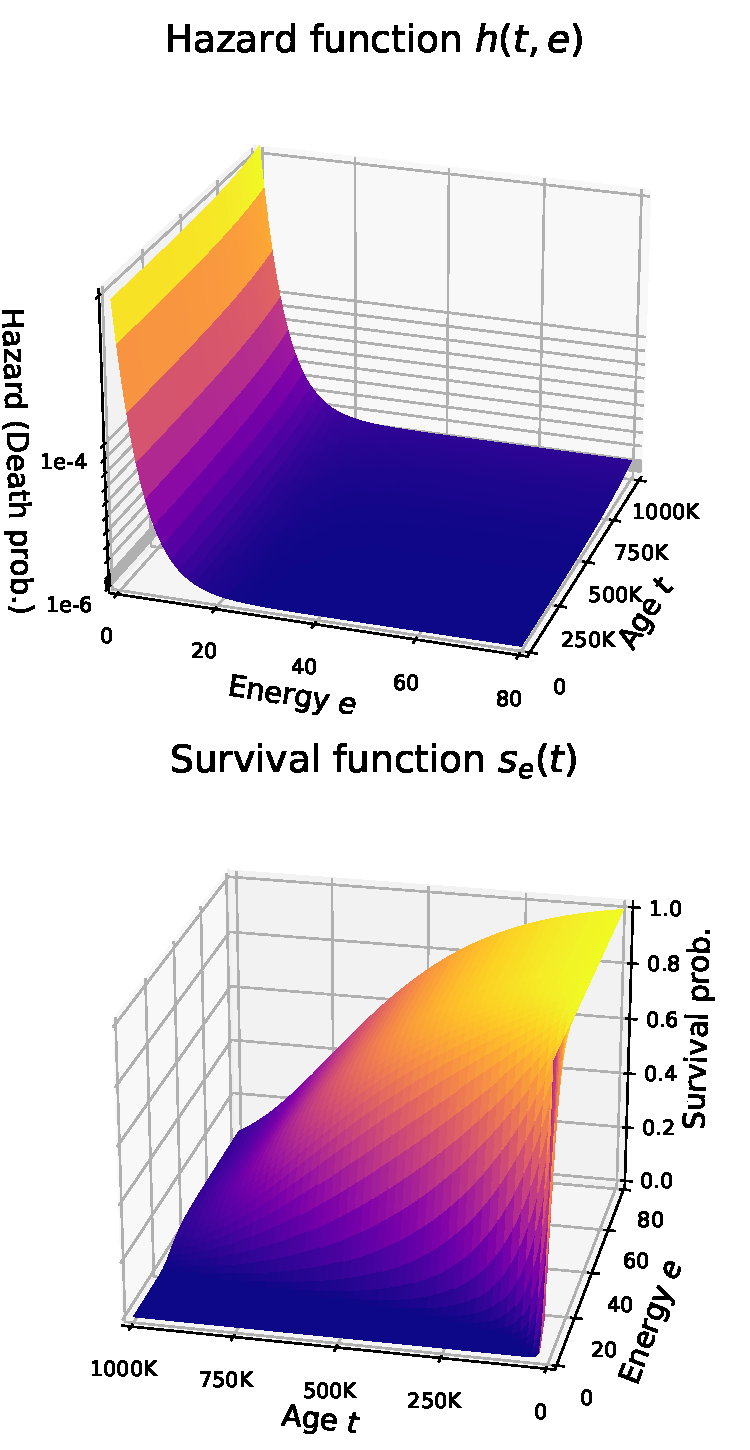
\includegraphics[width=15cm]{hazard_and_survival.pdf}
  \caption{
    \textbf{Left:} Designed hazard function $h(t)$ used for RL agents.
    \textbf{Right:} Survival function $S(t)$ corresponding to the hazard function.
  }\label{figure:hs}
\end{figure}

\paragraph{Energy-based death and birth model}
As a simple but biologically plausible way of simulating the birth and death of agents, we employ an energy-based model similar to \citet{hamonEcoevolutionaryDynamicsNonepisodic2023}. Each agent maintains their energy level $e$. Energy level $e$ increases by eating and decreases by primary metabolism and taking action in the environment. We design the agent's death and birth model to maintain a higher energy level $e$, which leads to longer lives and many offspring. With $e$ and an agent's age $t$, we let $h(t, e)$ be the hazard function for agents that evaluates the probability of an agent dying:

\begin{align}
  h(t, e) = \kappa_{h} \left(1 - \frac{1}{1 + \alpha_{he} \exp(\theta_{h} - e)} \right) + \alpha_{ht} \exp(\beta t). \label{eq:h}
\end{align}

This hazard function\label{eq:h} consists of two terms. The first term increases as energy levels decrease and follow a sigmoidal curve, where $\kappa_{h}, \theta_{h}$, and $\alpha_{he}$ are hyperparameters. The latter term $\alpha_{ht} \exp(\beta t)$ exponentially increases when the agent gets older, where $\alpha_{ht}$ and $\beta$ are hyperparameters. In population statistics, this is called the Gompertz hazard model\citep{gompertzXXIVNatureFunction1825,kirkwoodDecipheringDeathCommentary2015}. The left figure in \cref{figure:hs} shows the shape of the hazard function with the specific parameters used in our experiments. To intuitively understand the behavior $h$, we plot survival function $S(t, e) = \exp (-\int_{0}^{t}(h(t, e)) dt)$ in the right of \cref{figure:hs}. $S(t, e)$ is the probability for an agent to survive to the age $t$ if it keeps the same energy level $e$. We can see that the survival probability more sharply decays with aging when the energy level is low.

\begin{figure}[t]
  \centering{}
  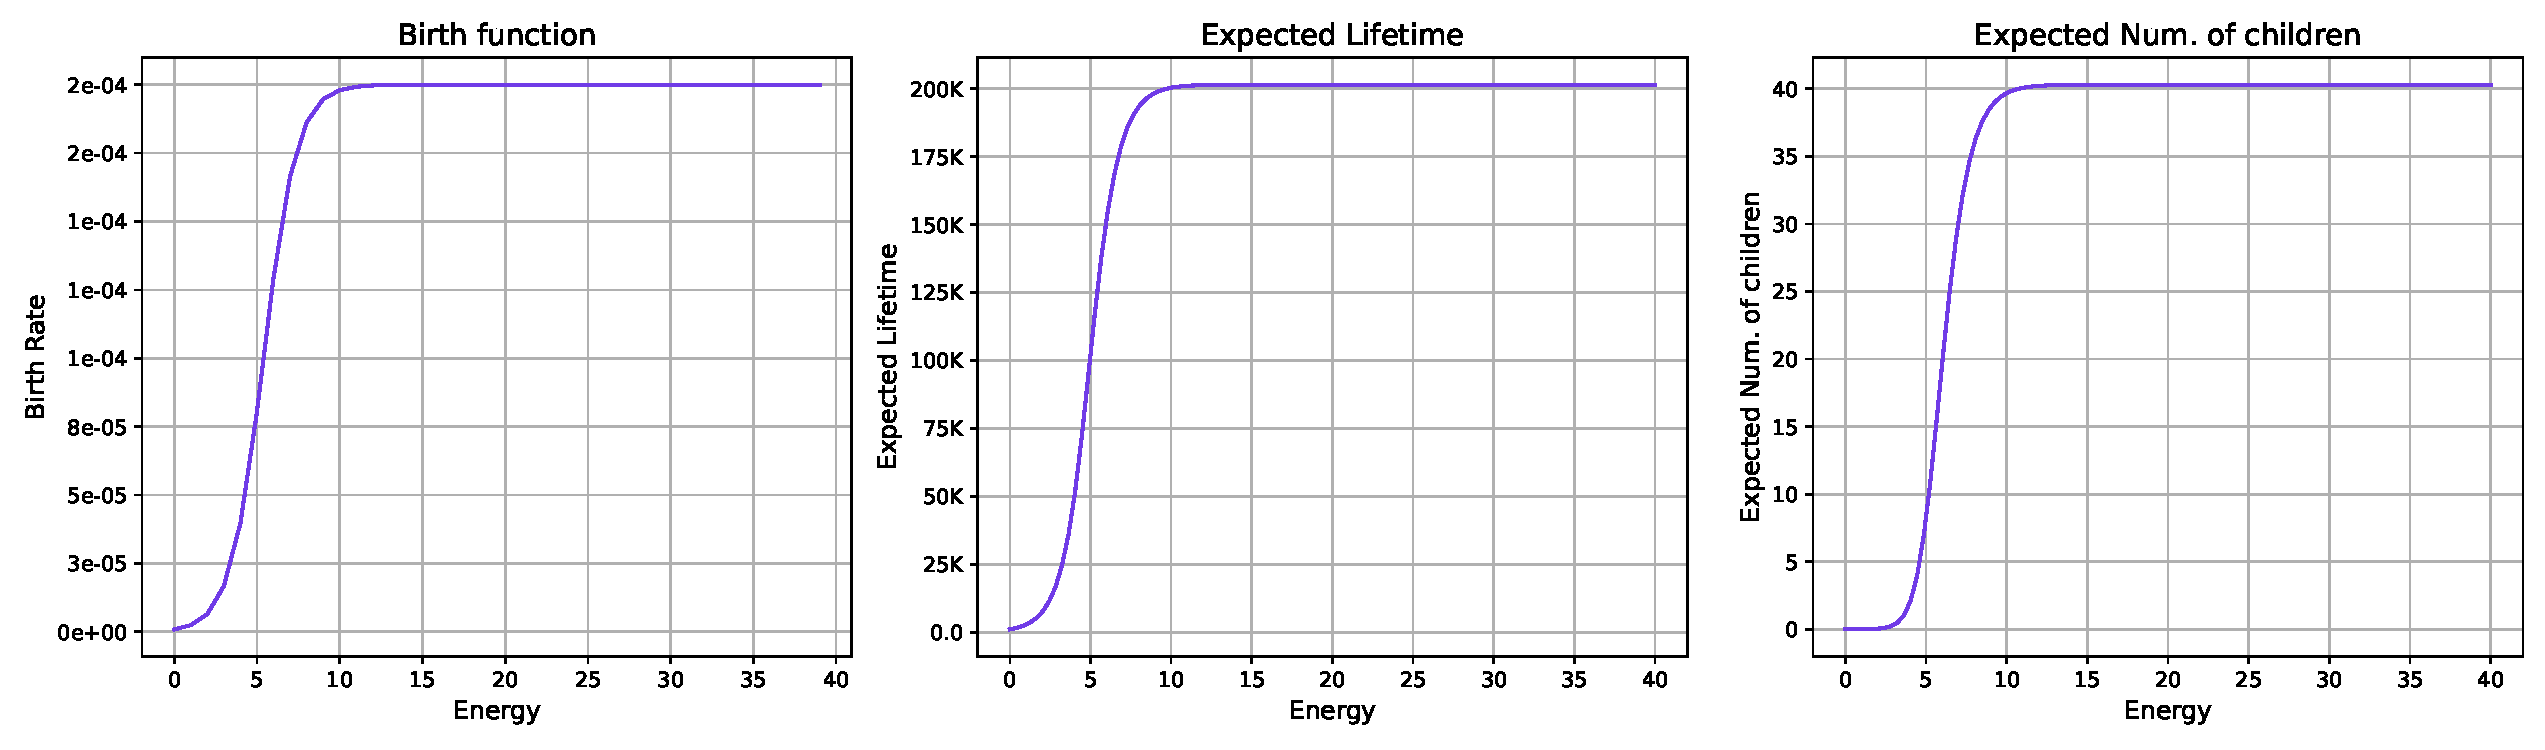
\includegraphics[width=15cm]{birth_and_nc.pdf}
  \caption{
    \textbf{Left:} Designed birth rate $b(e)$ for RL agents.
    \textbf{Center:} Expected lifetime for each agent
    \textbf{Right:} Expected reproduction number $R$ for RL agents corresponding to the designed hazard and birth functions.
  }\label{figure:bnc}
\end{figure}

For simplicity, we employ an asexual reproduction model where all agents can have a chance to make their children. We let $b(e)$ the birth function that evaluates the probability for an agent with energy level $e$ to make its child. Similarly to the first term of \cref{eq:h}, we design the birth function $b$ as:
\begin{align}
 b(e) &=  \frac{\kappa_{b}}{1 + \alpha_{b}\exp(\theta_{b} - e)}. \label{eq:b}
\end{align}
Modeled as a generalized logistic function \citep{richardsFlexibleGrowthFunction1959}, $b(e)$ increases with $e$ following a sigmoidal curve where $\kappa_{b}$ is the scale, $\theta_{b}$ controls the threshold of reaction, and $\alpha_{e}$ defines the shape of when $e = \theta_{b}$. The left figure of \cref{figure:bnc} shows the shape of $b$. For chosen $b$ and $h$, we plot the expected lifetime and number of children when an agent keeps the same energy level in the center and right figure in \cref{figure:bnc}. Parameters are chosen so that the maximum expected lifetime is around \num{200000} and the maximum expected number of children is around 40. All experiment parameters are shown in \cref{ap:param}.

\paragraph{Environment}

\begin{figure}[t]
  \begin{subfigure}[t]{6cm}
    \centering
    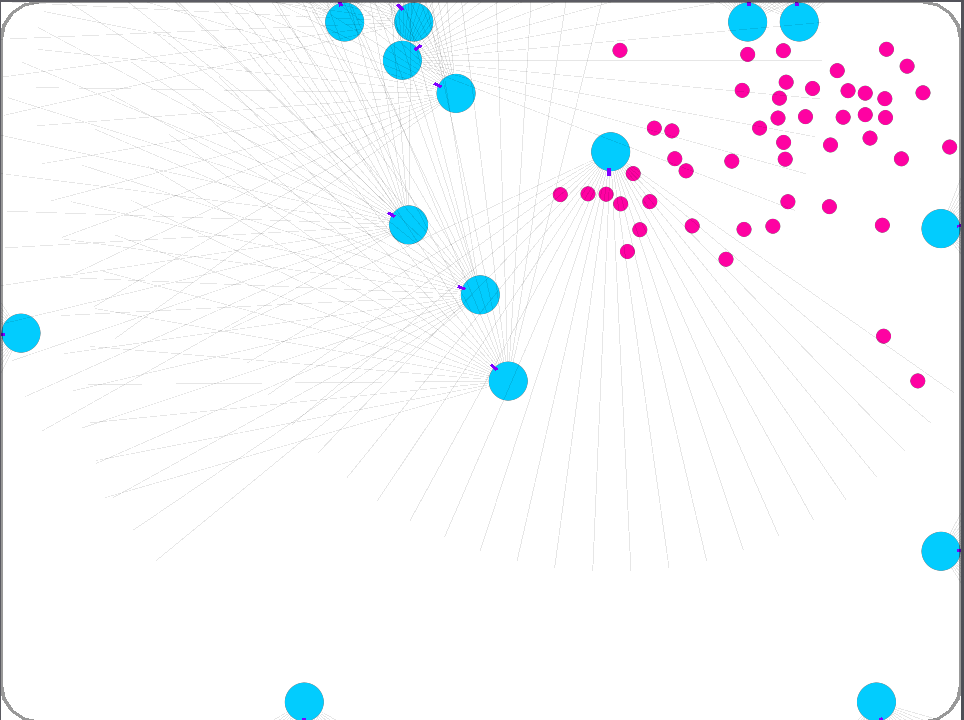
\includegraphics[width=6cm]{emevo-ss.png}
  \end{subfigure}
  \begin{subfigure}[t]{8cm}
    \centering
    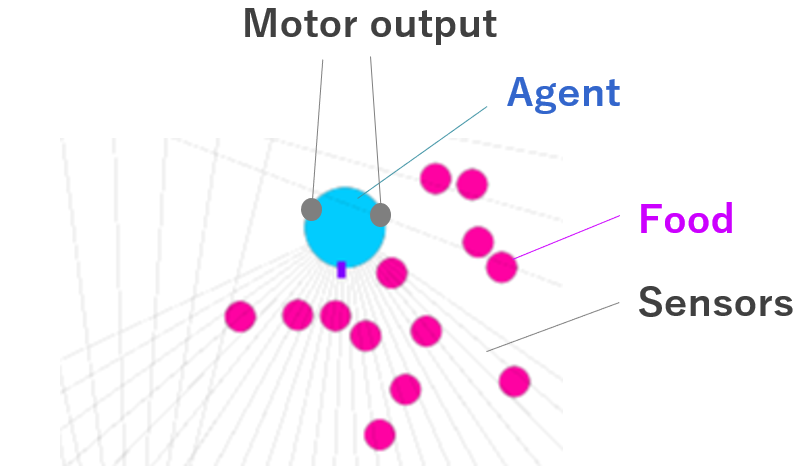
\includegraphics[width=8cm]{emevo-anno.png}
  \end{subfigure}
  \caption{
    \textbf{Left:} Environment.
    \textbf{Right:} Annotation
  }\label{figure:env}
\end{figure}

As a simple simulation environment with biologically plausible sensorimotor interaction, we design a continuous 2D environment shown in \cref{figure:env}. Blue circles indicate agents, and red circles indicate food. The environment is implemented by a 2D rigid-body physics simulation, and agents can move by adding motor outputs at two points in the diagonal back part of the circle. An agent can eat food by touching it. After foods are eaten, they are regenerated in a random place. The rate of food regeneration follows logistic growth function $\frac{dN_{food}}{dt} = r N_{food} (1 - \frac{N_{food}}{N_{food}^{\mathrm{max}}}$, where $N_{food}$ is the number of food, $r$ is growth rate, and $N_{food}^{\mathrm{max}}$ is the maximum number of food. Eating food increases

When an agent makes a child, a new agent is placed in a random location sampled from a Gaussian distribution centered around its parent. However, to speed up the simulation, reproduction fails when all sampled locations are not available. Thus, keeping away from other agents is beneficial for agents to make more children.
When the parent's energy level is $e$, a proportion of energy level $\eta e$ is given to the child and the parent lose it, where $\eta \in [0, 1]$ is the ratio of energy sharing. The child also inherits its reward function from the parent with some mutation.

Simulating many agents to maintain a reasonable size population (e.g., $50\sim 100$) is key in our evolution scheme. However, our preliminary CPU-based simulation experiments found that simulating collisions between many agents and foods could be a massive bottleneck in computation time. To overcome this challenge, we implement our environment using JAX Python library \citep{jax2018github} so that it can work on hardware accelerators such as GPU. Inspired by recent works on 3D rigid body physics simulation using JAX (e.g., \citet{brax2021github} and MuJoCo \citep{todorov2012mujoco} MJX\footnote{\url{https://mujoco.readthedocs.io/en/stable/mjx.html}}), we implement our 2D physics engine using JAX and build our environment on top of that. This design decision is made because many of the existing JAX-based physics simulation libraries are optimized for single-agent robot control and are not well suited for handling the multi-agent scenario we are dealing with. We explain implementation detail in \cref{ap:phys}.

\paragraph{Reward Function with Evolving Parameters}
We assume that the reward function is innate and cannot be changed by learning during an agent's lifetime. As sensory inputs that can affect reward function, we select \rnum{1} collision to food, \rnum{2} collision to the wall, \rnum{3} collision to some other agent, and \rnum{4} the magnitude of motor output. We expect that the reward for eating evolves from the collision to food and that the negative reward for fatigue evolves from the magnitude of motor output. Collision with the wall and other agents is chosen to test if the reward function can distinguish unrelevant signals for survival, as we do not penalize agents for colliding with walls or each other.

For ease of analysis, we model the reward for each sensory input separately. For example, the food reward is modeled as follows:

\begin{align*}
  r_{\mathrm{food}}^{t} =
  \begin{dcases*}
   10^{s_{\mathrm{food}}} w_{\mathrm{food}} & if the agent gets food at time t \\
   0 & otherwise
  \end{dcases*},
\end{align*}
where $s_{\mathrm{food}} \in [0, 1]$ and $w_{\mathrm{food}} \in [-1, 1]$ are evolvable parameters that represent scale and weight for the food reward. We model the reward for a collision to wall $r_\mathrm{wall}$ and other agents $r_\mathrm{agent}$ in the same way. Our intention in using two independent parameters is to balance stability and plasticity. Our preliminary experiments found that rewards can be too unstable if we allow significant change via a single parameter. Having a parameter for adjusting the scale separately makes the significant reward change more challenging while still possible. Similarly, letting $|a_t|$ be the Euclid norm of the action taken by agent at time $t$, the reward for taking an action is modeled by $r_{\mathrm{act}}^{t} = 10^{s_{\mathrm{act}}} w_{\mathrm{act}} c_\mathrm{act} |a_t|$, where $\eta_\mathrm{act}$ is a coefficient to adjust the scale of reward. Note that $r_{\mathrm{act}}^{t}$ is scaled so that it should have much smaller value than collision rewards, because an agent gets $r_{\mathrm{act}}^{t}$ every step while collision rewards are often $0$. The sum of these rewards $r_t = r_{\mathrm{food}}^{t} + r_{\mathrm{wall}}^{t} + r_{\mathrm{agent}}^{t} + r_{\mathrm{action}}^{t}$ is given to an agent for the use in RL.

\begin{algorithm}
  \caption{Reward evolution with asexual reproduction}\label{alg:reward-evo}
  \begin{tabular}{lll}
    \textbf{Input:} & $Pop, Env$ & Initial population and simulation environment\\
                    & $N$ & Number of rollout steps used in RL \\
                    & $h(t, e)$, $b(e)$ & Hazard and birth function for agents \\
                    & $mut(r)$ & Mutation function for reward function \\
                    & $\eta$ & Energy share ratio used in reproduction
  \end{tabular}
  \begin{algorithmic}[1]
    \Loop{}
    \ForAll{$agent \in Pop$}
      \State{$o \gets agent$'s observation in $Env$}
      \State{Sample an action $a$ from $agent$'s policy $\pi_{agent}(\cdot|o)$}
      \State{Update $agent$'s energy level $e$ based on the taken action $a$ and eaten food}
      \Once{in $N$ steps}
        \State{Update $agent$'s policy $\pi_{agent}$ and value function $\vh_{agent}$ via RL}
      \EndOnce{}
    \EndFor{}

    \State{Step the simulated environment $Env$ one step using collected actions}
    \LComment{Process death and birth}
    \ForAll{$agent \in Pop$ with energy level $e$, age $t$, and reward function $r$}
      \With{Probability $h(t, e)$}
        \State{$agent$ is removed from $Pop$ and $Env$}
        \Comment{agent is dead}
      \EndWith{}
      \With{Probability $b(e)$}
        \State{$e_\mathrm{new} \gets \eta e$, $r_\mathrm{new} \gets mut(r)$}
        \State{Add a new agent with reward function $r_\mathrm{new}$ and energy level $e_\mathrm{new}$ to $Pop$ and $Env$}
        \State{Update parent's energy to $(1 - \eta) e$}
      \EndWith{}
    \EndFor{}
  \EndLoop{}
\end{algorithmic}
\end{algorithm}

\paragraph{Simulation Procedure}
We show the pseudocode of our entire simulation procedure in \cref{alg:reward-evo}. 
This reward function uniform noise $[-0.1, 0.1]$ is added with probability $0.4$ to each element of $\mathbf{r}$. 
PPO\citep{schulmanProximalPolicyOptimization2017} as an RL algorithm because of its fast computation time.
Other RL-related parameters are put in \cref{tab:rl-param}.

\section{Results}

\section{Conclusion}

%\subsubsection*{Acknowledgments}\label{sec:ack}
% Use unnumbered third level headings for the acknowledgments. All acknowledgments, including those to funding agencies, go at the end of the paper. Only add this information once your submission is accepted and deanonymized.

%%%%%%%%%%%%%%%%%%%%%%%%%%%%%%%%%%%%%%%%%%%%%%%%%%%%%%%%%%%%%%%%
%% Bibliography
%%%%%%%%%%%%%%%%%%%%%%%%%%%%%%%%%%%%%%%%%%%%%%%%%%%%%%%%%%%%%%%%
\clearpage
\bibliographystyle{apalike}
\bibliography{references}

%%%%%%%%%%%%%%%%%%%%%%%%%%%%%%%%%%%%%%%%%%%%%%%%%%%%%%%%%%%%%%%%
%% Appendices
%%%%%%%%%%%%%%%%%%%%%%%%%%%%%%%%%%%%%%%%%%%%%%%%%%%%%%%%%%%%%%%%

% Retrieve appendix for arxiv?
% \clearpage
% \appendix
% \section{Implementation of 2D Physics in Jax}\label{ap:phys}
Our simulator implements projected Gauss-Seidel method with position correction \citep{catto2005iterative} that is fairly common in 2D game physics engines such as Box2D\footnote{\url{https://box2d.org}} and Chipmunk\footnote{\url{https://chipmunk-physics.net}}.

\section{Reward Function}\label{ap:reward}
As noted in \cref{sec:method}, we model reward weights for each sensory input by $r_{\mathrm{food}} = 10^{s_{\mathrm{food}}} w_{\mathrm{food}}, r_{\mathrm{agent}} = 10^{s_{\mathrm{agent}}} w_{\mathrm{agent}}, r_{\mathrm{wall}} = 10^{s_{\mathrm{wall}}} w_{\mathrm{wall}}$, and $r_{\mathrm{action}} = 10^{s_{\mathrm{action}}} w_{\mathrm{action}}$. For each collison events (e.g., collision to food), we let $c_{\mathrm{food}}, c_{\mathrm{wall}}$, and $c_{\mathrm{agent}}$ are

Similarly, letting $|a_t|$ be the Euclid norm of the action taken by agent at time $t$, the reward for taking an action is modeled by $r_{\mathrm{act}}^{t} = 10^{s_{\mathrm{act}}} w_{\mathrm{act}} c_\mathrm{act} |a_t|$, where $\eta_\mathrm{act}$ is a coefficient to adjust the scale of reward. Note that $r_{\mathrm{act}}^{t}$ is scaled so that it should have a much smaller value than collision rewards because an agent gets $r_{\mathrm{act}}^{t}$ every step while collision rewards are often $0$. The sum of these rewards $r_t = r_{\mathrm{food}}^{t} + r_{\mathrm{wall}}^{t} + r_{\mathrm{agent}}^{t} + r_{\mathrm{action}}^{t}$ is given to an agent for the use in RL.

\section{Environment Design}\label{ap:env}

\section{Hyperparameters}\label{ap:param}

\begin{table}[t]
  \centering
  \caption{Parameters for $h$ and $e$}\label{tab:bd-param}
  \begin{tabular}{ccl}
  \toprule
    Parameter & Value & Description \\
    \midrule
    $\kappa_{h}$ & 0.01 & Scaling parameter of the energy-related term in the hazard function \\
    $\alpha_{he}$ & 0.1 & Steepness of energy-related term in the hazard function \\
    $\alpha_{ht}$ & \num{1e-6} & Weight of the age-related term of the hazard function \\
    $\beta_{t}$ & \num{1e-5} & Steepness of age-related term in the hazard function \\
    $\kappa_{b}$ & \num{2e-4} & Scaling parameter for the birth function\\
    $\alpha_{b}$ & 0.01 & Steepness of the birth function \\
    $\theta_{b}$ & 10.0 & Reaction threshold for the birth function \\
    \bottomrule
  \end{tabular}
\end{table}

\begin{table}[t]
  \centering
  \caption{RL parameters}\label{tab:rl-param}
  \begin{tabular}{ll}
  \toprule
    Hyperparemeter & Value \\
    \midrule
    Discount factor ($\gamma$) & 0.999 \\
    PPO Rollout steps ($N$) & 1024 \\
    PPO Minibatch size & 256 \\
    PPO Number of optimization epochs & 4 \\
    PPO Clipping parameter & 0.2 \\
    PPO entropy coeff. & 0.0 \\
    GAE parameter ($\gamma$) & 0.95 \\
  \end{tabular}
\end{table}

We show all parameters used in our hazard model $h$ and birth model $b$ in \cref{tab:bd-param}.
We show all parameters used in our PPO implementation in \cref{tab:rl-param}.

\end{document}
\endinput
